\chapter{Experimental Results}


Implementation of details of  your project here. Implementation of details of  your project here. Implementation of details of  your project here. Implementation of details of  your project here. Implementation of details of  your project here. Implementation of details of  your project here. Implementation of details of  your project here. Implementation of details of  your project here. Implementation of details of  your project here. Implementation of details of  your project here. Implementation of details of  your project here. Implementation of details of  your project here. Implementation of details of  your project here. Implementation of details of  your project here. Implementation of details of  your project here. Implementation of details of  your project here. Implementation of details of  your project here. Implementation of details of  your project here. Implementation of details of  your project here. Implementation of details of  your project here. Implementation of details of  your project here. Implementation of details of  your project here. Implementation of details of  your project here. Implementation of details of  your project here. Implementation of details of  your project here. Implementation of details of  your project here. Implementation of details of  your project here. Implementation of details of  your project here. Implementation of details of  your project here. Implementation of details of  your project here. Implementation of details of  your project here. Implementation of details of  your project here. Implementation of details of  your project here. Implementation of details of  your project here. Implementation of details of  your project here. Implementation of details of  your project here. Implementation of details of  your project here. Implementation of details of  your project here. Implementation of details of  your project here. Implementation of details of  your project here. Implementation of details of  your project here. Implementation of details of  your project here. Implementation of details of  your project here. Implementation of details of  your project here. Implementation of details of  your project here. Implementation of details of  your project here. 

By doing so, we aimed to revolutionize the entire classification process, freeing educators from the burden of tedious manual data entry and empowering them to focus on more valuable tasks in education.
, which can be a pioneering step towards comprehensive document classification

\section{System Description}

Our system uses a camera to accept images as input as per our requirements. This obtained input is then processed using the \textbf{img2table} library. Using this library, the cell coordinates are extracted and cropped to obtain the values inside the cell. These values are then given to the TensorFlow OCR model to accurately classify and predict the values obtained from the cell extraction step. The obtained result from this step is arranged specially in the format of CSV files.

\section{Existing Solutions}

\noindent
Since there is no available research journal that emphasizes the complete working of our system, we discuss the literature review in detail by exploring how each research paper contributed to the creation of our system.

\noindent
When we initially formed our idea, we wanted the idea to be projected in a way that helps reduce the teacher's efforts the most. Our initial sources of the study were Google Lens and Microsoft Lens, but since they are closed-source software, we could not rely on them to understand how the backend of both those applications works. 

\clearpage

\noindent
On thorough research, we found that the base idea behind all this is optical character recognition (OCR). Aaryan Raj et al. [1] proposed {\it Revolutionizing Data Entry: An In-Depth Study of Optical Character Recognition Technology and Its Future Potential} in February 2023. 

\noindent
It provides a comprehensive analysis of the history, current state, and future of OCR technology. By the concluding statements of this research journal, we decided to make OCR the main focus of our project.

\noindent
Most of the OCR technologies work by taking images as input variables. But how we do this process was our next dilemma. What our project required was the front page of the answer sheet and the table of marks on that page, specifically speaking the cells are to be extracted separately. Colin G. White-Dzuro et al. [7] proposed {\it Extracting Medical Information from Paper - COVID-19 Assessment Forms} in 2021. It examines the validity of optical mark recognition, a novel user interface, and crowd-sourced data validation to rapidly digitize and extract data from paper COVID-19 assessment forms at a large medical center. Here, we observed a technique where they extract only the important feature cells from a COVID-19 assessment form, which we assumed was applicable in our case. But after discussion with the team, we were able to conclude that this was not practically difficult as our answer scripts will have varied patterns of mark arrangement depending on how the questions are answered or how many subdivisions a question has. Also, the paper also warns that their proposed model is prone to errors and only guarantees an accuracy of 70\%. Thus we needed to explore other techniques which is when we found out about table detection methods.

\noindent
Jiayi Yuan et al. [8] proposed {\it An OpenCV-based Framework for Table Information Extraction} in September 2020. It proposes a novel OpenCV-based framework to extract the metadata and specific values from PDF tables. B.Gatos et al. [14] proposed {\it Automatic Table Detection in Document Images} in 2005. It proposes a workflow for table detection that comprises three distinct steps: (i) image pre-processing; (ii) horizontal and vertical line detection and (iii) table detection. Here, they discuss the Probabilistic Hough Line Transform \textbf{(houghlinesp())} in the OpenCV package which can be used to create a bounding box around the desired cells that we need to extract. 

\clearpage

\noindent
Also, they discussed an alternate option in contour functions that can work as a line joining all the points along the boundary of an image that are having the same intensity. When we tested our sample dataset against Hough Line Transform, we will identify and separate pixels based on their color range. So we decided to use this library for the next step of our project.

\noindent
With this, we were able to mold the initial concept of our project. We take in our images as input, we pass it through the table recognition/detection after which we perform OCR on the image data. This OCR-processed data is then obtained as final output in a CSV file. The concept is clearly depicted in Figure 2.1.

\begin{figure}[h!]
    \centering
    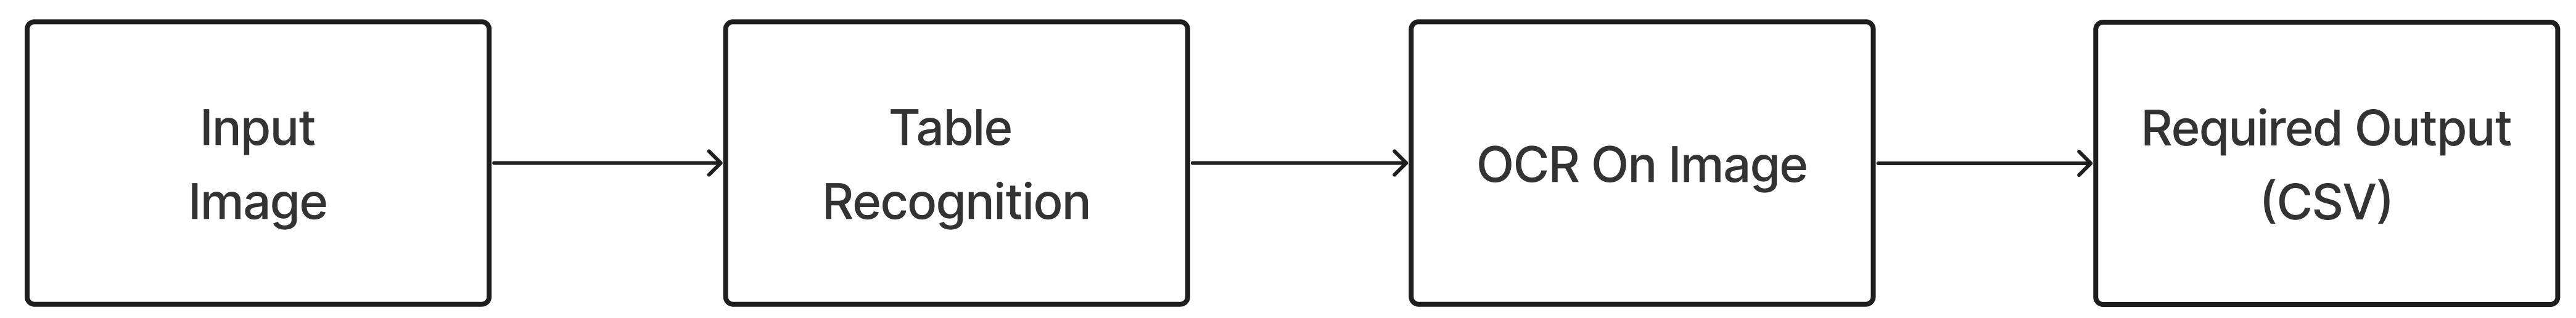
\includegraphics[width=1\textwidth]{Images/lit_review/Initial concept of our system.png}
    \caption{Initial concept of our system}
\end{figure}



\noindent
The next process that we needed to handle was how to build our OCR model. Abhishek Das et al. [9] proposed {\it LSTM-based  Odia  Handwritten  Numeral Recognition} in September 2020. It focuses on the loss in recognizing the digits and is evaluated using the categorical cross-entropy loss function and for optimization, we have applied Adam optimization to minimize the error. The approach in focus here is LSTM\nomenclature{LSTM}{Long Short Term Memory} while Raajkumar G. et al. [11] proposed {\it Optical Character Recognition using Deep Neural Network} in July 2020. It aims at analyzing various text images like blurred and tilted images and it identifies the text from these images using deep learning models. The approach in focus here is CNN.

\noindent
While under research about neural network, we discovered Chen ShanWei et al.[6] proposed {\it A CNN-based Handwritten Numeral Recognition Model for Four Arithmetic Operations} in 2021. It proposes an automatic checking system based on CNN for handwritten numeral recognition. By the concluding statements of this journal, we were able to confirm that CNN must be the backbone concept of our project. In future scope implementations, we would suggest adding layers of LSTM to compare the difference between the previous and updated versions of the model.

\clearpage

\noindent
Ömer Aydin [4] proposed {\it Classification of Documents Extracted from Images with Optical Character Recognition Methods} in June 2021. It focuses on the fact that handwriting or printed documents have been digitalized by a scanner or digital camera and these documents have been processed with two different OCR operations. Sachin Shrivastava et al. [5] proposed {\it CNN-based Automated Vehicle Registration Number Plate Recognition System} in March 2021. It focuses on the different methods of VRNPR\nomenclature{VRNPR}{Vehicle Registration Number Plate Recognition} and emerging technologies that are used to get accurate results. Both these research papers helped us gain a little more perspective and understanding of how CNN can be applied to real-life scenarios and situations of the most importance. 

\noindent
In the midst of doing all this research, we also planned out our data collection procedure. We shared the progress of our project with our guide regularly and also borrowed answer scripts from our department with the authorization of our head of department. The dataset we were able to create from these answer scripts was too small, overall we have only cell images between 700-800 in number with each class attaining a bare 70-100 range of images. So we decided to explore methods in which we could implement CNN with a very small dataset. Bjorn Barz et al. [12] proposed {\it Deep Learning on Small Datasets without Pre-Training using Cosine Loss} in May 2020. It shows that the cosine loss function provides substantially better performance than cross-entropy on datasets with only a handful of samples per class. We obtained a large dataset of number images from Kaggle, and combining that with our original dataset, we tested it with the cosine loss function. According to the TensorFlow documentation, it is possible to apply the sparse categorical cross-entropy function. This is made possible because the labels for the number images stored in the folders have the same names as the folders themselves.

\noindent
With all the information that we collected up til now, and all the data we had in store, we were able to build a working model for our project using CNN. The main users for this project would be our teachers who would want to use an application that appeals to them as easy and simple to use. So we decided to explore the options to build an interface with a suitable front-end framework. Akkem Yaganteeswarudu [10] proposed {\it Multi Disease Prediction Model by using Machine Learning and Flask API} in July 2020. 

\clearpage

\noindent
It focuses on Python pickling, which is used to save the model behavior, and Python unpickling, which is used to load the pickle file whenever required. Using the conclusion from this paper, we decided to move forward and create an interface using Flask API. We were able to make the interface look quite simple and unique to our project objectives.

\begin{figure}[h!]
    \centering
    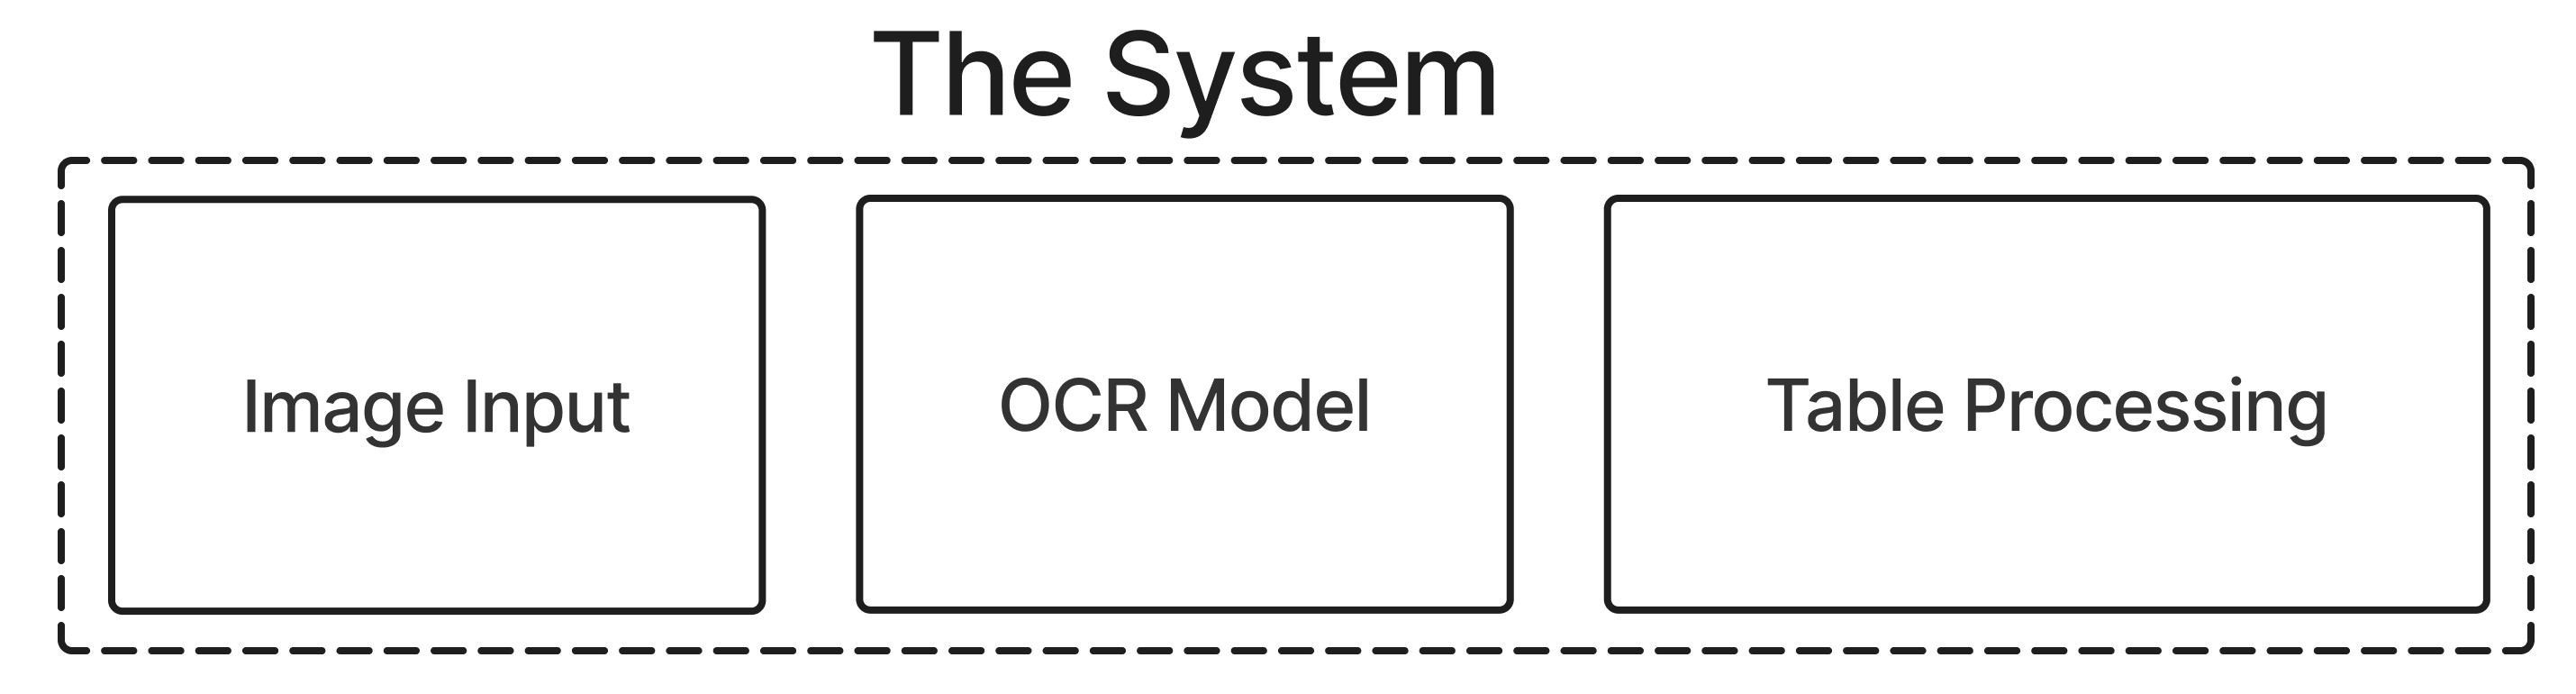
\includegraphics[width=0.8\textwidth]{Images/lit_review/main_components_of_MP.jpg}
    \caption{Main components of our system}
\end{figure}

\noindent
Figure 2.2 shows the main components of our system. In overall, we can summarize our project in three stages \begin{enumerate}
        \item Preparation of image dataset 
        \item Creation of OCR model 
        \item Table recognition and real-time prediction
    \end{enumerate}. 

\vspace{2.5mm}

\noindent
In the initial stage of image input, we can do it in two methods: real-time camera feed and PDF upload. Uploading camera feed images in real time is a cost ineffective strategy and the reasons for this are that it needs good background lighting, a fixed angle setting and camera picture quality. On the other hand, uploading PDFs would be much easier and practical to many who possess standard quality cameras. But we must also note that the quality of PDF images would vary from device to device and small deviations like skew and symmetry values would result in the model not functioning as per our requirements.

\noindent
The next step is the model creation. Here, we train our model with the obtained dataset and enhanced its performance by frequently changing parameters to test changes in model performance. We save the model in \textbf{.h5} format and it performs much better when compared to other model versions as we change the .h5 models. This feature helps in the easy plug-in and plug-out of the whole model.

\clearpage

\noindent
The final step is table recognition. At present, we have designed this section of the system specifically according to the SJCET answer sheet format. If another institution wishes to use our system, they can modify the table recognition module of the system and customize it according to their institution's answer sheet format. We have designed this system to be open-source and customizable for different users' needs.

\section{Summary}

\noindent 
Initially, the aim was to develop a system that would assist teachers in reducing their workload by automating the extraction of marks from answer scripts. Various options were explored, including gaining an understanding of the inner workings of Google Lens and Microsoft Lens. However, the focus was later shifted to (OCR) technology.

\noindent
After conducting further research, a combination of OCR and table detection techniques was deemed suitable for extracting marks from answer scripts. It was discovered that the \textbf{img2table} library outperformed the Hough Line Transform algorithm from OpenCV for table detection. Consequently, the decision was made to opt for img2table for table detection.

\noindent
The next step involved building an OCR model. At first, the CNN and LSTM network architectures were considered, but ultimately, the decision was made to go with CNN as it was a simpler and more straightforward option to begin with. The CNN model was trained on a dataset of handwritten digits, which included samples from both answer scripts of the college and an open online handwritten-numbers dataset from Kaggle.

\noindent
Additionally, a user interface for the system was developed using the Python Flask API. The interface is designed to be simple and user-friendly, enabling users to access the camera for capturing images of answer scripts and subsequently downloading the extracted marks in a CSV file.
